










\begin{figure}[!h]
	\centering     %%% not \center

	\subfigure[a]{ \label{fig:a}
		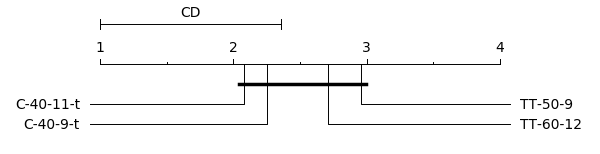
\includegraphics[width=70mm]{conteudo/capitulos/figs/CDs/WinDiff.png} }	
	\subfigure[b]{ \label{fig:b}
		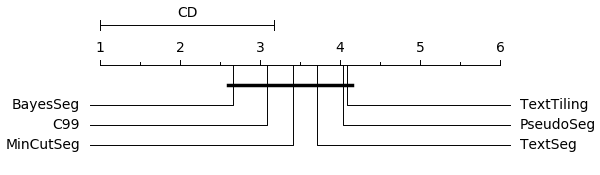
\includegraphics[width=70mm]{conteudo/capitulos/figs/CDs/Pk.png} }
	\subfigure[c]{ \label{fig:c}
		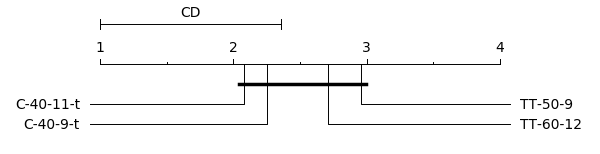
\includegraphics[width=70mm]{conteudo/capitulos/figs/CDs/Acuracy.png}}
	\subfigure[d]{ \label{fig:d}
		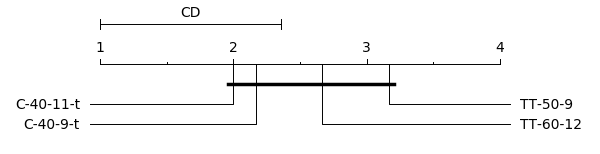
\includegraphics[width=75mm]{conteudo/capitulos/figs/CDs/Precision.png}}
	\subfigure[e]{ \label{fig:e}
		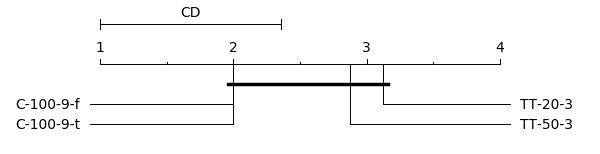
\includegraphics[width=70mm]{conteudo/capitulos/figs/CDs/Recall.png}}
	\subfigure[f]{ \label{fig:f}
		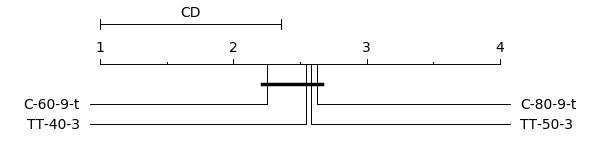
\includegraphics[width=70mm]{conteudo/capitulos/figs/CDs/F1.png}}

		\caption{Diagramas de Diferença Crítica sobre \textit{ranking} dos algoritmos de segmentação baseados em coesão léxica de acordo com valores de \textit{WindowDiff}, $P_k$, Acurácia, Precisão, Revocação e $F^1$.}
	\label{fig:CDs}
\end{figure}







  \begin{center}
	\begin{figure}[h!]

		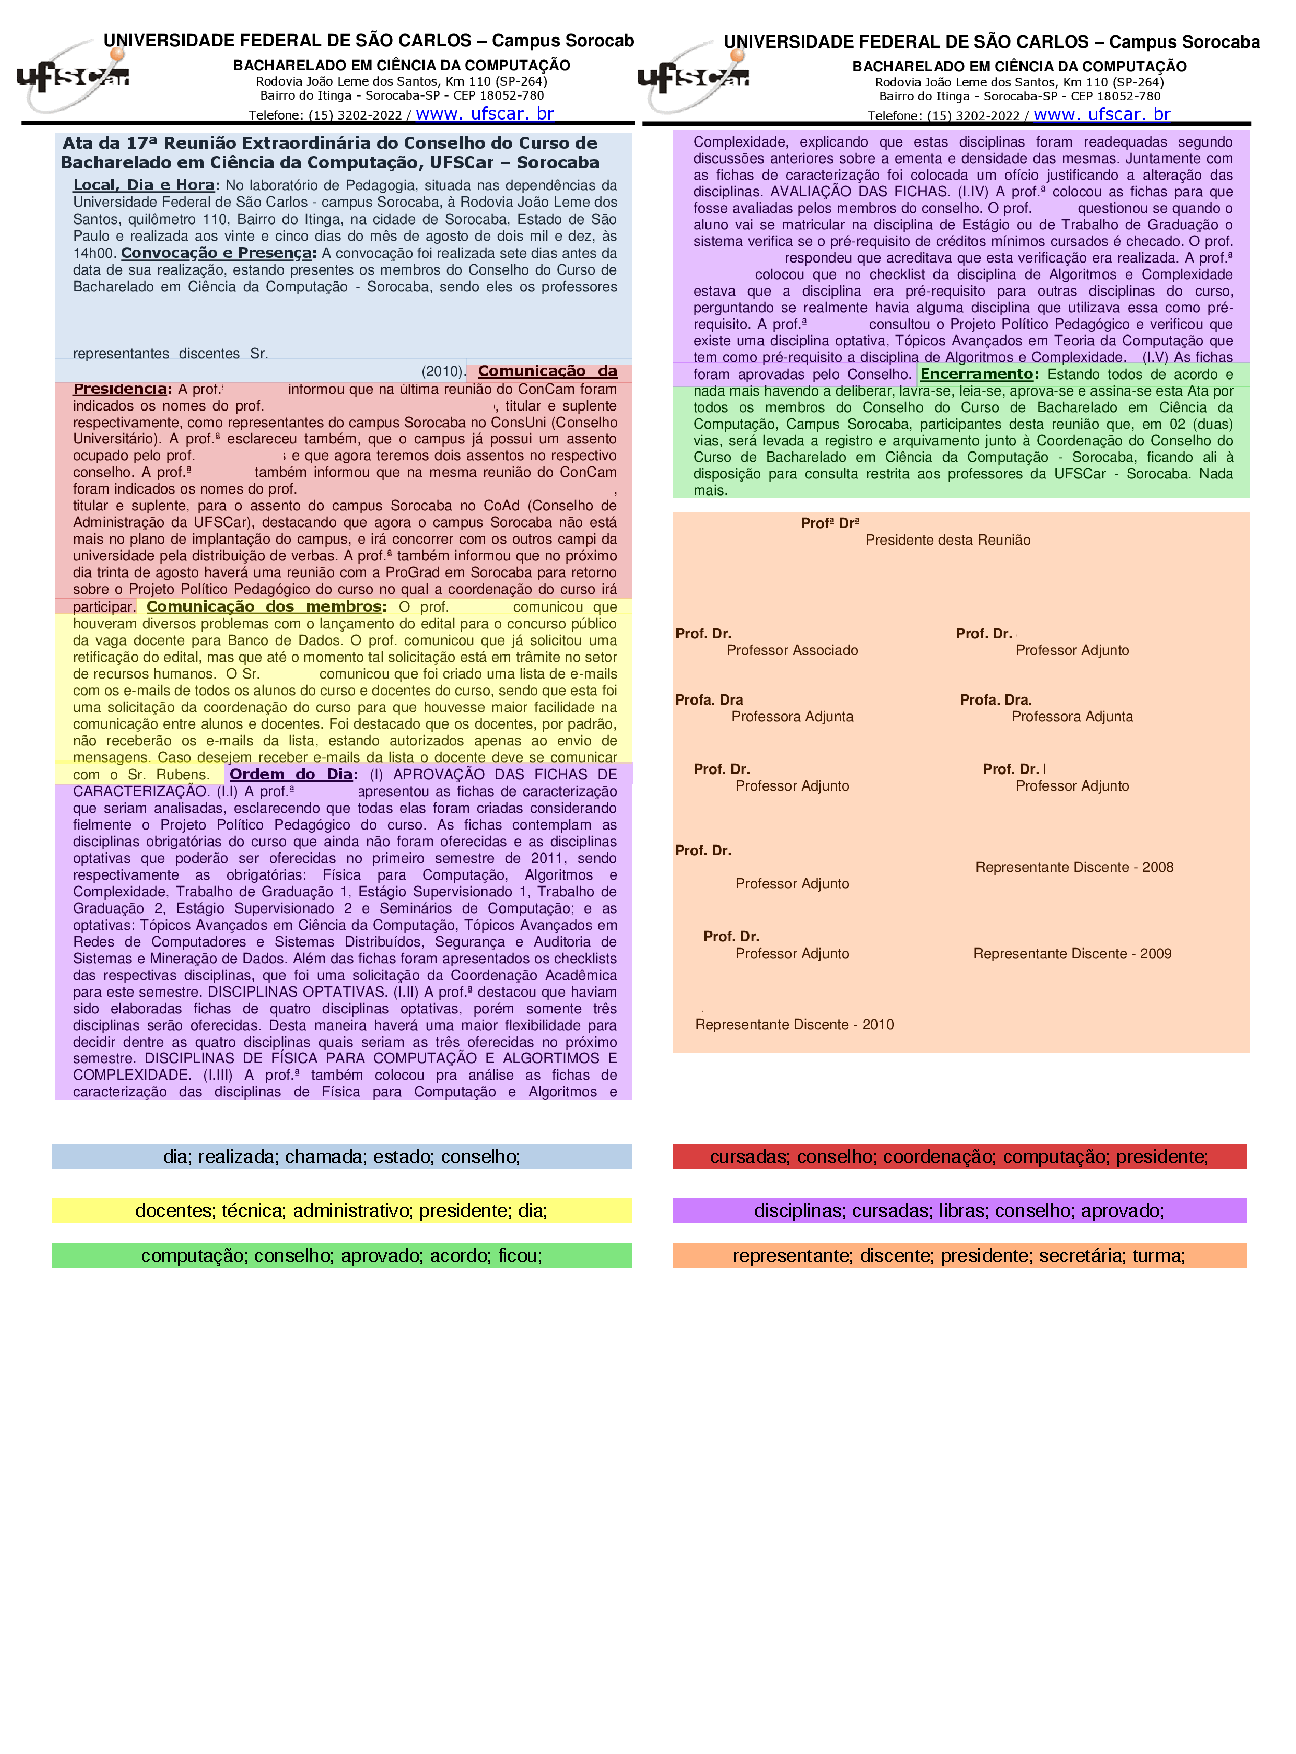
\includegraphics[trim={ 0 235 0 0 },clip,page=1,width=\textwidth]{conteudo/capitulos/figs/doc-em-png/distribuicao.pdf}

	\end{figure}
\end{center}


\label{fig:distribuicao-ata}

\caption{Distribuição de tópicos em uma ata real. Cada tópico é representado por uma região colorida. Abaixo estão os descritores identificados pela cor do respectivo tópico. Os nomes de pessoas foram ocultados por não expressarem significado nesse trabalho.}





Informações contidas em grandes quantidades de texto;
Grandes volumes de texto com conteúdo irrelevante;
Documentos desestruturados;
Dificuldade em resgatar essas informações manualmente;


	\item Uma atas registra vários assuntos;

Motivação:
\begin{itemize}
	\item São fontes de consulta e utilizadas como referência e apoio a decisões; 
	\item Um assunto pode ser discutido diversas vezes em reuniões diferentes;
	\item É desejável recuperar um histórico dessas decisões ao longo do tempo;
	\item Necessidade de ferramentas automáticas;
\end{itemize}

Motivação:


Atas de reunião registram os assuntos tratados  como base de dados


\item Contém segmentos de texto com assuntos relativamente independentes; 



- Incapacidade humana em gerenciar grandes volumes de documentos;








Fiz um roteiro com:
Motivação
Objetivos
Proposta
Resultados
e Conclusão


acho que é esse roteiro mesmo
mas tipo
os "trabalhos relacionados"
meio que vão aparecer na motivação
pq vc vai falar que tem alguns estudos que segmentam determinados tipos de texto
mas não o que vc vai trabalhar lá em específico





hora que for explicar abordagem proposta
vc vai explicando cada etapa do seu framework
e lá vc vai mostrando a teoria envolvida com cada parte












A literatura apresenta abordagens 


Essa tarefa tem 2 passos principais:
\begin{itemize}
	\item Encontrar pontos onde há transição de assuntos;
	\item Identificar esse assunto;
\end{itemize}







Visão Geral 
imagem segmentação 
imagem documento com tópicos identificados nos segmentos



  % \begin{figure}[!h]
  % \centering
  % 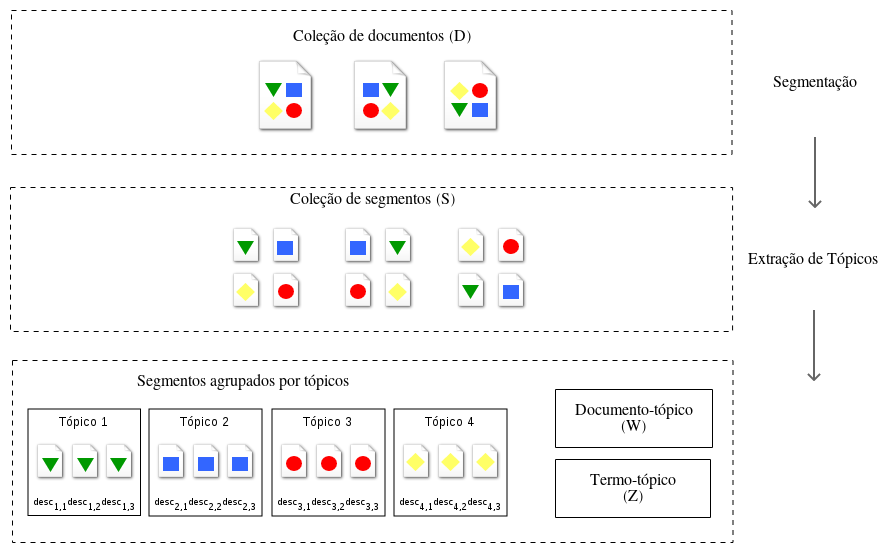
\includegraphics[width=.8\paperwidth]{images/estrutura.png}
  % \caption{Estrutura de dados interna e seu processo de geração.}
% %  \label{fig:#4}
  % \end{figure}





% \nblock{}{
\begin{itemize}
	\item Propor uma solução para identificar, organizar e consultar assuntos registrados em atas de reunião.  
	\item Utilizar técnicas de Segmentação textual em conjunto com modelos de Extração de Tópicos para:
		% \nblock{}{
			\begin{itemize}
	\item Gerar uma estrutura mais organizada que a coleção original.
	\item Utilizar a estrutura latente dos segmentos para Recuperação de Informação. 
		\end{itemize}
		% }
	% \item Dar início a investigação dessa abordagem no contexto de atas de reunião.
\end{itemize}
% }










o objetivo desse trabalho de mestrado é propor o 





desenvolvimento uma ferramenta 


para identificar, organizar e apresentar assuntos registrados em atas de reunião 


utilizando a estrutura latente de documentos segmentados em conjunto com técnicas de recuperação de informação.





% Propor uma solução para encontrar porções de texto relevantes à consulta.






